\chapter{Requirements}


\section{Scenario}
Software deployment tools play an important role in continuous integration and automation.
It is imperative that these tools are easy to use and flexible in many scenarios.
A typical pipeline normally responds to changes in code, triggered by a version control
system. A number of steps must be executed before new code reaches production machines to
ensure that changes are safe to deploy and that they can be reverted if needed.

A typical pipeline may include a code source, build process, test execution, packaging,
revision storage and retreival and finally deployment. The system should be flexible to
allow deployment in various configurations such as single developer machines, remote
machines and fleets of machines in round robin, waves, one then all or all together.

The goal of the project is to provide an easy to use framework for creating a code
deployment pipeline. Third party developers should be able to extend the capabilities
of the system through the provided interception points.

The framework comes with a pre-packaged server so that clients need only register their own or
third party integrations and start the server. The server provides a REST API allowing
clients to see and create pipelines as well as add and configure modules at various
interception points provided by the framework. The client may also see the status of the
pipeline.

The framework allows the client to register an endpoint with a version control system,
such as GitHub. When changes are made GitHub can trigger the execution of the pipeline.

\section{Use Cases and Use Case Descriptions}
  \subsection{Use Case Diagram}
    \begin{figure}[H]
        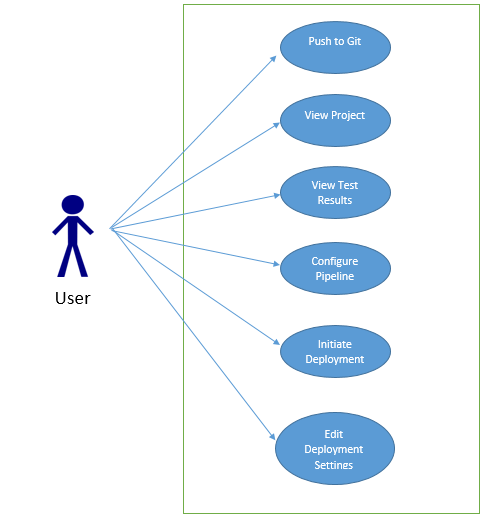
\includegraphics[width = 1.2\linewidth]{diagrams/UseCaseDiagram}
        \caption{Use Case Diagram}
        \label{fig:use_case_diagram}
      \end{figure}

   \subsection{Use Case Description}
   \begin{figure}[H]
       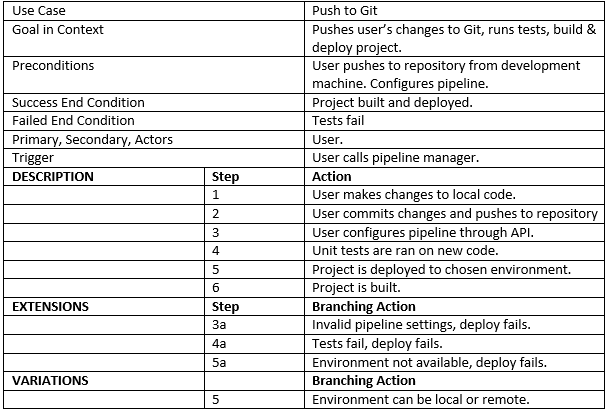
\includegraphics[width = 1.2\linewidth]{diagrams/DetailedUseCase}
       \caption{Use Case Description}
       \label{fig:use_case_description}
     \end{figure}


\section{Non-Functional Requirements}

In software systems, non-functional requirements (NFRs) describe how a system works, while functional requirements describe what the system should do. Unlike functional requirements, NFRs are not captured in use cases and cannot be analysed by drawing sequence diagrams or state charts. Non-functional requirements can be subjective and can be evaluated differently by different people. For these reasons, NFRs can be difficult to deal with. Yet, dealing with NFRs can be vital for the success of a software system. \cite{nfrs} Failing to meet a non-functional requirement can result in systems that fail to satisfy business and user needs or can result in unfulfilled mandatory requirements imposed by regulatory or standards agencies. NFRs usually cannot be implemented in a single module of the system and can be categorised into 3 main types according to Gorton (2006) \cite{sw-arch}:
\begin{itemize}
  \item Quality attributes / architectural use cases e.g. ``ilities"
  \item Business e.g. FDA standard compliant
  \item Technical e.g. must develop in Python and use Flask microframework
\end{itemize}

\subsection{Security}
Software security protects systems from unintended and unauthorized access and protects against malicious attacks and other risks, so that the software can continue to function correctly under such potential risks. Encryption is the most effective way to achieve data security. During user authentication, the user's credentials (username and password) should be encrypted so that they can be transferred over the framework securely. The encrypted values can then be compared with encrypted information in the database.

Audit logs should be verbose enough to support forensics. All account modification events as well as any system warnings or errors should be logged and monitored. This can be supported using the Interceptor design pattern. An example event log after a system modification would include information such as date, time, user, action, entity changed, prior value and new value. Web-based issue trackers could also provide a way for users of the framework to report bugs and vulnerabilities. Such reported vulnerabilities should only be accessible by individuals with prior permission from the security team.

\subsection{Extensibility}
Good architectural design is supported by system components that can be extended easily by both the developer of the framework to create new versions of the components and by third-parties (users) that have to adapt components for use in specific software systems. Good extensibility in a software system can be achieved by architectural design patterns such as the Abstract Factory and the Interceptor. Using an object-orientated language such as Python helps with the implementation of design patterns. The deployment framework being developed will most likely feature glass-box extensibility. This refers to a software system that may be extended with third party extensions that are separate from the original framework in a way that does not affect the original framework. The clean separation of the framework and the third-parties' extensions makes it easier to understand and maintain extensions. \cite{glassbox}

\subsection{Performance}
Performance is a measure of the amount of work accomplished by a computer system. High performance involves a system having short response times, low utilisation of computing resources (compute, storage, networking), high availability and short data transmission time. Performance can be improved by distributing work across multiple machines in the system. Types of work that could be distributed for a deployment framework include builds/testing, deployments and database utilisation across disks (NoSQL databases give up some features of the traditional databases for speed and more importantly for horizontal scaling).

\subsection{Configuration Management}
Configuration management is the task of tracking and controlling changes in a system. If a failure occurs in a system due to an incorrect configuration, configuration files can determine what was changed and who changed it. Distributing text files containing configuration information is a common way to manage configurations in a software system. Master copies of important configuration files are kept in a central location and distributed to machines that require them. Centralization enables version control, reducing the time taken to make changes across large groups of hosts. Using a simple version control system such as Git will ensure any config changes are logged and can be audited if the need arises.

Ansible and Chef are examples of configuration management tools. Both tools achieve similiar results but work in different ways. Chef operates on a client-server model, where a Chef server stores configuration files called Cookbooks. The client nodes run the Chef client software, which performs the automation and config management upon receiving instructions from the Chef server. On the other hand, Ansible is agentless, requiring nothing on target hosts systems other than SSH and Python. This makes Ansible easy to work with and has excellent inbuilt security with SSH.


\section{Tactics to Support Architectural Use Cases}

Any software system design consists of a collection of decisions. A tactic is a design decision that influences the control of a quality attribute response. A collection of tactics are called an architectural strategy. For example, an architect might employ rendundancy and synchronization to support availability in a software system. \cite{sw-arch-2}

\subsection{Modifiability}
Modifiability is the time and cost associated with implementing, testing and deploying changes to a software system. Restricting modifications to a small set of modules will generally reduce the modification cost. During design, we assigned responsiblities to modules such that anticipated changes would be limited in scope. Given the nature of a software framework, all of the framework-side implementation is non-modifiable by the client. This also helps to prevent ripple effects, the necessity of making changes to modules after a modification. The use of configuration files for the interceptors also localized the changes needed when configuring the deployment of a application.

\subsection{Portability}
We used the Python language for the implementation of the code deployment framework. Python is a widely used interpreted language that emphasizes code readability. It features a dynamic type system and supports object-orientated programming. Python comes preinstalled on most Linux distributions and python interpreters are available for many operating systems, allowing Python code to run on a wide variety of systems. The use of virtual environments and the Pip package manager during testing and deployment allowed us to simplify dependency management, making it very easy to move our software from one environment to another.

\subsection{Extensibility and Flexibility}
The interceptor pattern implements serveral tactics to support extensibility in a software system. By customising and configuring interceptor and dispatcher interfaces, users of a concrete framework can add, change and remove services without knowledge of the concrete framework architecture or implementation. In the case of our code deployment framework, users can add interceptors for various stages in sourcing, building, deploying and storing application code. Interceptors can be added transparently without affecting existing application code becuase they are decoupled from application behaviour.